\section{Supervised approach} \label{supervised_approach}

Our second approach to performing \acrshort{si} in the repositories is based on using external data to train a machine learning classifier, which will then be applied on the documents of the repositories. In machine learning, this field is called \acrfull{hmc}, as a variable number of labels may be assigned to any object, and the labels are organized in a hierarchy. The relevant literature was presented in chapter \ref{hmc}. The main challenge of the supervised approach is that the data used to train the classifier is noisy. The authors of \acrshort{mag}, whose data we are using, estimate that their subject indexing procedure has an accuracy of 80 \%.

This approach is fundamentally opposite to the unsupervised approach, which uses only data present in the repositories. The word embeddings and the vocabulary used in this approach are independent of the repositories, meaning that this classifier could be used without any modifications for any repository whose documents are topically similar to the ones used to train the classifier. This is an important difference between the approaches in terms of applicability, as the unsupervised approach is tailored specifically for our dataset, including numerous data cleaning steps and exception handling that are hard to generalize for their use in different scenarios.

Given that this approach should be widely applicable, we use pre-trained word embeddings. We present different in section \ref{supervised_approach_embeddings}. In the end, we use the fastText embeddings \cite{mikolov2017advances} because of their high accuracy and their similarity to the ones we trained ourselves in the unsupervised approach.

We then present and analyze the data we have gathered to train the models in section \ref{supervised_approach_data}. We have retrieved 200,000 documents from OpenAlex, each with a title, an abstract and a set of assigned subjects. As we want our training data to be well distributed across our subset of \acrshort{mag} subjects, we have retrieved up to 100 documents per subject.

In section \ref{supervised_approach_models}, we discuss our model architecture, which we have adopted from a similar use case \cite{gargiulo2019deep}. It includes two convolutional layers for feature extraction and two fully connected layers that compute assignment probabilities for each subject, given a document. We also implement two further extensions of the model. The first one only modifies the loss function to account for the imbalance between positive and negative samples in multi-label scenarios \cite{ben2020asymmetric}. The second one further extends the loss function by ensuring that the assignment probabilities don't violate the subject hierarchy \cite{giunchiglia2020coherent}. This enforcement is also performed by an additional layer we append to the first model.

We thus have three models. They all use the same neural network architecture, excepting the coherent model, which adds another layer on top. The main difference between the models is the loss function. Finally, in section \ref{supervised_approach_conclusion}, we talk about different aspects of this approach, such as its complexity and its computational cost. In summary, this approach is easy to implement but expensive to compute, as optimizing its parameters involves extensive experimenting. We also discuss potential improvements, such as modeling the label noise or introducing the confidence scores into the model.

\subsection{Embedding model} \label{implementation_skipgram}

To transform text into vectors, we first embed words into vector space. We could do so randomly, but this wouldn't take into account the semantic information of the words. To preserve this information, we use skip-gram \cite{mikolov2013distributed}, a word embedding model. This model was also used by \acrshort{mag} in their procedure. We already gave an overview of its design in section \ref{mag_skipgram}. In this section, we will look at how we trained the model and some examples of the resulting embeddings.

We train 100-dimensional word vectors, which we initialize with values sampled from the uniform distribution bounded by -1 and 1. The word vectors of \acrshort{mag} comprise 250 dimensions. We have decided to use fewer dimensions given that our vocabulary is much smaller: it includes around 50,000 entries, whereas \acrshort{mag}'s vocabulary has than 2 million.

We trained the model for 8 epochs. Surprisingly, it reached its best epoch loss already in the second iteration. The model optimized the embeddings quickly during the first epoch, starting with a batch loss of $30$ and ending with an average epoch loss of $4.9$. Figure \ref{fig:loss_avgs} shows the avg. loss of each epoch. Figure \ref{fig:loss_avgs_range} also shows the avg. loss, but with bars illustrating the range of the batch losses throughout the epoch.

\begin{figure}
  \begin{subfigure}[t]{0.5\textwidth}
    \centering
    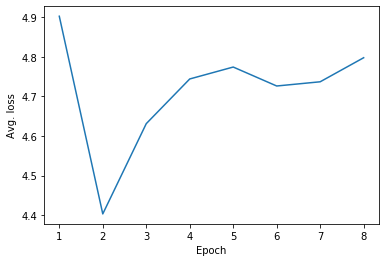
\includegraphics[width=\textwidth]{figures/unsupervised_approach/loss_avgs.png}
    \caption{Avg. training loss of each epoch.}
    \label{fig:loss_avgs}
  \end{subfigure}
  \hfill
  \begin{subfigure}[t]{0.5\textwidth}
    \centering
    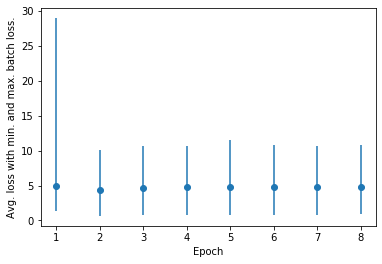
\includegraphics[width=\textwidth]{figures/unsupervised_approach/loss_avgs_range.png}
    \caption{The dots refer to the avg. epoch loss, while the extrema of the line refer to the min. and max. batch loss of that epoch.}
    \label{fig:loss_avgs_range}
  \end{subfigure}
  \caption{Plots of the training loss of the skip-gram model.}
\end{figure}


\subsubsection{Resulting embeddings}

We have computed the cosine distance between certain words to serve as an example. The cosine distance is also the metric we use to compare subjects and documents. The results can be found in table \ref{tab:embeddings_examples}. We have chosen three pairs of words, each of a different field. `polymer'' and ``monomer'' belong to the realm of chemistry; ``machine'' and ``learning'' usually refer to a family of algorithms; ``magnetic'' and ``resonance'' refer to a medical procedure. The chemistry pair is fed to the skip-gram model 96 times during training; the computer science pair, 1357 times and the medicine pair, 961 times.

Given that the cosine distance is symmetric, we only show one half of the table. Also, the distance of a vector to itself is zero. The table shows that the pairs of words of each field are closer to each other than to the other words. The distance between ``polymer'' and ``monomer'' is the largest of the three, which makes sense, as the model receives this pair of words hundreds of times less than the two others. The smallest distance between words that do not belong to the same field is between the words ``magnetic'' and ''polymer''. This distance is 34 \% larger than the distance between ``monomer'' and ``polymer''. Thus, the word vectors accurately differentiate between words that belong to the same field and those that don't.

As a further example of the semantic expressiveness of the embeddings, we can look at the word ``program'', although it belongs to the same field as the computer science pair, it is not as closely related to them. In fact, it appears 27 times as an input to the model with either of the words ``machine'' and ``learning''. However, this is more often as for the pairs of chemistry and medicine, with which it appears as input 26 and 3 times, respectively. The model was able to identify that ``program'' should be closer to the computer science pair, even if it appeared only one time less with the chemistry pair. Its cosine distance to ``machine'' and ``learning'' are 0.77 and 0.72, respectively. On the other hand, its cosine distance to the rest of the words is above 1.

\begin{table}[]
    \centering
    \begin{tabular}{c|c c c c c c}
       $dist(x,y)$ & monomer & polymer & machine & learning & magnetic  \\
       \hline
       resonance & 0.96 & 0.91 & 0.95 & 0.95 & \textbf{0.21} & \\
       magnetic & 0.88 & 0.82 & 0.98 & 0.98 & & \\
       learning & 1.08 & 1.19 & \textbf{0.41} & & & \\
       machine & 1.02 & 0.95 & & & & \\
       polymer & \textbf{0.54} & & & & & \\
    \end{tabular}
    \caption{Cosine distances between the vectors of certain words. The distances of words of the same field are highlighted in bold.}
    \label{tab:embeddings_examples}
\end{table}
\subsection{Training data} \label{supervised_approach_data}

In this section, we present the subset of \acrshort{mag} documents, which we use to train the supervised models. We first present how we have retrieved documents from the OpenAlex \acrshort{api} in section \ref{supervised_approach_data_retrieval}. We retrieve up to 100 documents for each subject in our subset, ensuring that each document has an abstract.

Then, in section \ref{supervised_approach_data_hierarchy}, we analyze the subject assignments of the documents. We focus on the consistency of the assignments regarding the hierarchy. If a document is assigned a subject, it should also have all its ancestors assigned. This is relevant for the model training, as hierarchy violations hinder the model's understanding of the subjects \cite{gargiulo2019deep}.

Finally, in section \ref{supervised_approach_data_result}, we discuss the resulting dataset. We have gathered over 200,000 documents. After correcting hierarchy violations, it comprises almost 2 million subject assignments. Only two subjects are not assigned to any documents, out of the 2,157 included in our subset.

\subsubsection{Document retrieval} \label{supervised_approach_data_retrieval}

To retrieve documents from OpenAlex, we iterate over the subjects in our subset of \acrshort{mag} subjects and look for journal articles that include each subject. We iterate over the resulting documents, and keep those that have an abstract and were not previously retrieved through another subject. The abstract of the documents is given as an inverted index, where each word is mapped to its positions in the abstract. This was done for copyright reasons.

We have retrieved up to 100 documents per subject, and stored them in multiple files, with max. 3,000 documents per file. For each document, we first build the abstract and append it to the title. We then process the resulting text, and store it in a file together with its assigned subjects. The processing involves tokenizing and lemmatizing the data, just as it was done for the texts of the repositories (see section \ref{implementation_vocab}). We also discard stopwords and tokens that have less than three letters, which removes numbers, symbols and quantities (e.g. 100mg).

\subsubsection{Hierarchy violations} \label{supervised_approach_data_hierarchy}

Here we look at the subject assignments of the documents presented above, looking for inconsistencies regarding the hierarchy of subjects, before presenting the final training dataset. The assignments of a document are inconsistent if the ancestors of an assigned subject are not assigned as well. We consider this a violation of the hierarchy.

There are 1,952 documents that are not assigned a \acrshort{mag} field, which are therefore inconsistent, as they are assigned subjects of further levels but not from the first. Interestingly, 122 of these documents have the subject \textit{Mechanics} assigned to them. 427 of these documents without assigned fields only have one assigned subject. On average, these subjects are assigned 1.2 subjects, with 1,582 distinct subject assignments. We have corrected these violations using the lists of ancestors of the subjects. The resulting dataset is presented in the next section.

\subsubsection{Resulting dataset} \label{supervised_approach_data_result}

\begin{figure}
    \centering
    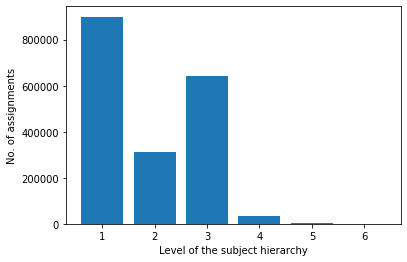
\includegraphics[width=.7\textwidth]{figures/supervised_approach/training_data_levels.png}
    \caption{Number of subject assignments per hierarchy level.}
    \label{fig:training_data_levels}
\end{figure}

Following the retrieval procedure outlined above, we could gather 214,538 documents, comprising 100 documents for all subjects except for 17. When looking at all assignments, there are two subjects of our subset for which we could not retrieve any documents: \textit{Algorithm design} and \textit{Premise}. There are two further subjects for which we could not retrieve any documents (\textit{Shoot} and \textit{Intensive care unit}), but they are present in more than 300 documents each, when looking at the whole dataset. This occurs because the only documents that include these subjects were already retrieved by looking at the documents assigned with other subjects.

In total, there are 1,890,080 subject assignments. 821,273 of these assignments were added to fix hierarchy violations. The field that has benefited the most from fixing the hierarchy violations is \textit{Engineering}, which went from being the field with the least assignments (2,565), to having over 60,000 assignments. All fields have more than 20,000 assignments after the corrections, whereas before there were several with less than 5,000 assignments.

As shown in \ref{fig:training_data_levels}, most of them belong to the first hierarchy level. Here, only the field assignments are considered. \textit{Biology} is the most assigned field, with over 80,000 assignments. \textit{Art} has the least assignments, with just over 20,000. Among the other levels of the hierarchy, the most popular subjects are \textit{Law}, with 49,842 assignments and \textit{Ecology}, with 37,136 assignments. Both had less than 10,000 assignments before fixing the hierarchy violations.

Although we have avoided duplicates by keeping the OpenAlex IDs of the retrieved documents, there are 4,849 documents with the same data. 122 of them are documents for which no tokens remained after the filtering procedure, and 31 of them have uninformative texts like review appeals. The remaining documents are actual duplicates, with the same data appearing in at most three documents. There are 2,346 distinct documents among them, with an average of one duplicate per document. Thus, the final number of distinct documents is 212,035.

\begin{figure}
    \centering
    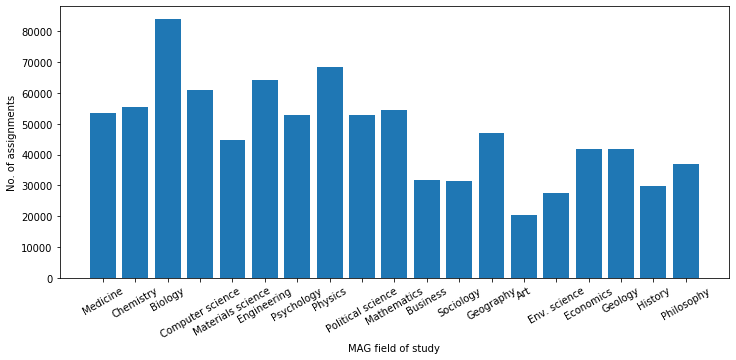
\includegraphics[width=\textwidth]{figures/supervised_approach/training_data_fields.png}
    \caption{Distribution of the documents across the MAG fields of study.}
    \label{fig:training_data_fields}
\end{figure}
\subsection{Our classifiers} \label{supervised_approach_models}

We implement the convolutional neural network detailed in \cite{gargiulo2019deep}, as their use case closely resembles ours (see section \ref{hmc_gargiulo}). They also work with scientific texts and assign to them subjects organized in a hierarchy. The paper provides a complete architecture, from processing the text, to extracting features and feeding them to a classifier. Their architecture is grounded on previous work, which makes their design decisions more sound. Our use cases differ mainly in three points:

\begin{enumerate}
    \item \textbf{Training data}: they have over eleven million documents, two orders of magnitude more than us.
    \item \textbf{Label noise}: their subject indexing procedure was performed by humans, whereas ours was performed by an unsupervised algorithm, which is not as accurate.
    \item \textbf{Subject hierarchy}: theirs comprises more than 20,000 subjects, one order of magnitude more than us.
\end{enumerate}

We consider these differences when adapting the architecture for our case. We discuss the design choices of the original architecture and the changes we have made in section \ref{supervised_approach_design}. These include reducing the size of the model, given our smaller number of labels and our shorter inputs, increasing the dropout probability, which was very low in the original implementation, and using a learning rate schedule instead of keeping it constant.

In section \ref{supervised_approach_add_asymmetry}, we replace the loss function of our model with one specifically designed for \acrfull{mlc} \cite{ben2020asymmetric} that decouples positive from negative labels, which allows the model to focus on the rare positive samples instead of on the numerous negative ones. See section \ref{hmc_asl} for more details. This loss function was used in \cite{zhao2021evaluating} to evaluate \acrshort{mlc} with noisy labels, concluding that it increased the regularization of the model, thus avoiding overfitting the noisy data. Therefore, this loss function may help us address label noise, the second difference between the original use case and ours.

The second extension we implement is the addition of the \acrlong{mcm} and using the \acrfull{mcl} \cite{giunchiglia2020coherent} as our model's loss function. To the best of our knowledge, it is the current \acrshort{sota} for \acrshort{hmc}. The paper was already presented in section \ref{hmc_forward}. Given that both the \acrshort{asl} and the \acrshort{mcl} extend the \acrshort{bce}, we combine them, yielding the \acrlong{aml}, which we use for this model.

We thus have three models. They only differ on the loss function, and the additional layer of the coherent model. All other model parameters, as well as the training settings, are the same. For brevity, we refer to each of the three models by their loss function: the \acrshort{bce} model, the \acrshort{asl} model and the \acrshort{aml} model. We present their architecture and parameters in the following sections.

\subsubsection{Design of the classifying pipeline} \label{supervised_approach_design}

\begin{figure}
    \centering
    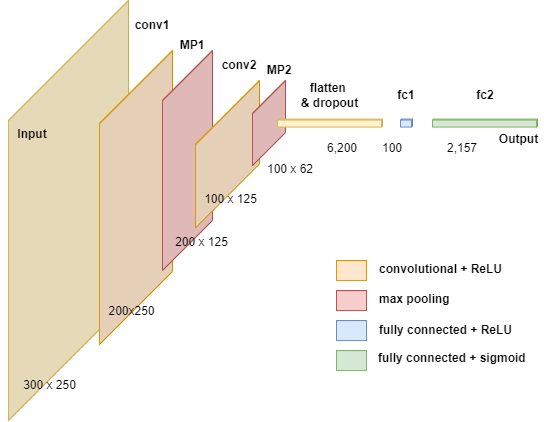
\includegraphics[width=.85\textwidth]{figures/supervised_approach/model_diagram.png}
    \caption{Diagram of the model. The shown sizes are the outputs of each layer.}
    \label{fig:model_diagram}
\end{figure}

Our model comprises two phases: one where feature extraction is performed, and a second one where the probabilities of each subject being assigned to the input document are computed. We first define the input to the model, which is not the same as for the original implementation (i.e. the one from \cite{gargiulo2019deep}), given our different use cases. We use only one representation type instead of four, and we keep the first 250 words of each text, instead of the first 400. Then, we explain the architecture of the model. We adapt the original implementation to our use case, and also optimize several aspects through experimentation. Please note that a description of how convolutions are applied to text was given in section \ref{hmc_cnn}.

\paragraph{Input} \mbox{}

The input to the model is a collection of word vectors. In the original implementation, they pick the first 400 words of each text and discard the rest. If a text has less than 400 words, they pad it with zero vectors. As shown in figure \ref{fig:sm_doc_length}, most of our documents have less than 250 tokens. We therefore pick 250 as our threshold, and also pad when necessary. Some representations are very short because the documents don't have abstracts, or because they are written in other languages and tagged as they were in English (see section \ref{repo_analysis_data}).

We only consider the tokens for which we have a pre-trained vector. The fastText word vectors are 300-dimensional, meaning they comprise 300 floating numbers each. Thus, the input is formed by 250 word vectors, each with 300 dimensions. As shown in figure \ref{fig:model_diagram}, the input forms a matrix, where each word vector is a column.

\begin{figure}
    \centering
    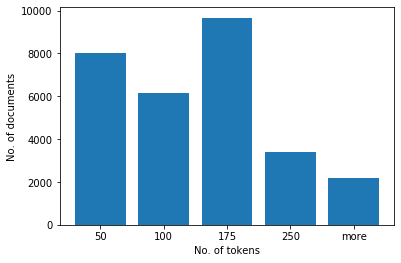
\includegraphics[width=.6\textwidth]{figures/supervised_approach/sm_doc_length.png}
    \caption{No. of tokens per document, in five groups.}
    \label{fig:sm_doc_length}
\end{figure}

\paragraph{Model architecture} \mbox{}

The feature extraction phase comprises two convolutional layers, each followed by ReLU activation and a max-pooling layer. Both pooling layers have a kernel size of 2, and both convolutional layers have stride 1. The stride defines the steps taken across the input between convolutions. Furthermore, both convolutional layers use padding to keep the number of dimensions unaltered

The first convolutional layer has 200 filters and kernel size 5. The number of filters is the number of features extracted from the input. Thus, the resulting matrix has 200 rows and the same number of columns, as shown in figure \ref{fig:model_diagram} in the \textit{conv1} layer. The kernel size defines how large a context window should be considered for each word vector. The second convolutional layer has 100 filters and kernel size 3. The resulting matrix, which comprises 100 rows and 62 columns, is flattened into a one-dimensional vector. Then, its constituent elements are zeroed with a certain dropout probability, a regularization technique used to avoid overfitting. The probability of this layer is discussed in the following section.

The assignment probabilities for each document are computed by a classifier consisting of two fully connected layers. The size of the output is equivalent to the number of subjects, as we want to output an assignment probability for each of them. The output layer also has sigmoid activation instead of ReLU, so each probability is between zero and one. The size of the first layer, called the hidden layer, comprises 1,024 neurons in the original paper, as their number of subjects exceeds 20,000. Given that our set of subjects is one order of magnitude smaller, we have reduced the size of the hidden layer. We experiment with 100 and 200 neurons in appendix \ref{supervised_approach_optim}. As both values perform similarly, we keep the lower one for further regularization and less computational cost.

\subsubsection{Training parameters} \label{supervised_approach_params}

The model parameters are optimized using \acrfull{sgd}, where the gradient is estimated by considering only a subset of the data. It is a trade-off between computational cost and fast convergence rate, parameterized by the batch size. A larger batch size accelerates convergence (regarding the number of steps), but also increases the computational cost. The original implementation uses a batch size of 10 and improve the convergence rate with a Nesterov momentum of $0.5$. Momentum introduces inertia into the gradient space, meaning that the direction of the steps are influenced by previous steps. They use \acrfull{bce} as a loss function. As discussed in section \ref{hmc_asl}, this is the common loss function for multi-label settings.

We experimented with two different sizes for the hidden layer: 100 and 200. The results showed that both sizes performed similarly. We decided to keep the lower size, which reduces the computational cost and increases regularization. We also experimented with two values for the dropout probability which were common in the literature: 30 \% and 70 \%, concluding that the higher value offers better results. The original implementation used a dropout probability of 10 \%, which is very low when compared with the literature. Both experiments can be found in appendix \ref{supervised_approach_optim}.

Interestingly, the original implementation doesn't use a learning rate (LR) scheduler, which is common practice in deep learning. Instead, they keep the LR constant at $0.1$. This is not optimal, both in terms of efficiency and accuracy. Gradient steps should be larger when further away from the optimum, to increase convergence rate, and decrease over time to not overshoot the optimum. Our experiments, presented in appendix \ref{supervised_approach_optim}, show that the 1-cycle policy fits our use case better than a decaying LR schedule. Cyclical LR schedules \cite{smith2017cyclical} follow the observation that increasing the LR may lead the model to perform better in the long term. The 1-cycle policy increases the LR until it reaches a given maximum, and then decreases it monotonically afterwards.

\subsubsection{Adding asymmetry} \label{supervised_approach_add_asymmetry}

Our first extension of the model described above, which we term \acrshort{bce} model because of its loss function, is to replace its loss function with the \acrfull{asl}, resulting in the \acrshort{asl} model. The \acrshort{asl}, which was already presented in section \ref{hmc_asl}, extends the \acrfull{bce} loss to address the imbalance between positive and negative samples in multi-label settings. It receives two parameters, $\gamma_-$ and $\gamma_+$. They modulate the importance of negative and positive samples, respectively. The larger their values, the lower the impact of their corresponding samples on the result of \acrshort{asl}.

We have experimented with these parameters in appendix \ref{supervised_approach_asymmetric}, concluding that the optimal values for our use case are $\gamma_+=1$ and $\gamma_-=2$. Recall that the \acrshort{asl} model is exactly the same as the \acrshort{bce} model, except for the loss function.

\subsubsection{Adding coherence} \label{supervised_approach_add_coherence}

The second extension of the \acrshort{bce} model is the addition of a new layer, called the \acrfull{mcm}, and the use of the \acrfull{aml}. The \acrshort{mcm}, which was presented in section \ref{hmc_forward}, enforces the subject hierarchy upon the output of the model, so subjects have an assignment probability at least as high as the assignment probabilities of their descendants. In practice, the \acrshort{mcm} is implemented as a matrix, where each row has ones for the subject it represents and its descendants, and zeros otherwise. Each row of this matrix is multiplied element-wise with the output of the model. Then, the maximum of each row is assigned to the corresponding subject.

The loss function used by the original coherent model \cite{giunchiglia2020coherent}, called the \acrfull{mcl}, modifies \acrshort{bce} loss to also ensure that the assignment probabilities respect the subject hierarchy. Given that the \acrshort{asl} also extends  \acrshort{bce}, we can combine them. Below is a comparison of all three loss functions, and their resulting combination, which we term \acrfull{aml}. In these formulas, $D(x)$ is the set of subjects that are descendants of subject $x$. All the individual losses are then averaged to arrive at the final loss for a document, which has as many of these input-output pairs as there are subjects.

\begin{align*}
    & BCE(x, y) = -y \cdot \log (x) - (1-y) \cdot \log (1-x) \\ \\
    & ASL_{\gamma_-, \gamma_+}(x, y) = -y \cdot \log (p) \cdot (1-p)^{\gamma_+} - (1-y) \cdot \log (1-p) \cdot p^{\gamma_-} \\ \\
    & MCL(x, y) = -y \cdot \log (\max(x, \{x_d \cdot y_d, \forall d \in D(x)\}) - (1 - y) \cdot \log (1 - MCM_x) \\ \\
    & AML_{\gamma_-, \gamma_+}(x, y) = -y \cdot \log (\max(x, \{x_d \cdot y_d, \forall d \in D(x)\}) \cdot (1-p)^{\gamma_+} \\
    & \qquad \qquad \qquad \qquad - (1 - y) \cdot \log (1 - MCM_x) \cdot p^{\gamma_-} \\
\end{align*}

We have performed an experiment to compare the \acrshort{mcl} with the \acrshort{aml}, outlined in appendix \ref{supervised_approach_coherence}, concluding that \acrshort{aml} performs better in our dataset. We thus use the \acrshort{aml} in our third supervised model.
\subsection{Conclusion} \label{supervised_approach_conclusion}

We conclude this chapter by discussing the complexity of the implementation and some aspects of the model that may be improved to increase the performance of the model. The implementation of the models, as well as gathering the training data, is easy to develop. On the other hand, processing the training data training the models is computationally expensive.

We propose several improvements, mostly regarding the fact that the subject assignments are performed by an algorithm and not by a human. This means that its assignment noise could be modeled more easily, as the algorithms operates in a deterministic manner, whereas humans are not so consistent. Also, the assignment algorithm outputs confidence scores, which could also be used to improve the training procedure.

\subsubsection{Implementation}

The supervised approach was easy to implement. Gathering the training data didn't pose any difficulties because of the \acrshort{api} provided by OpenAlex. We vectorized the data in the same way we vectorized the documents of the repositories. Implementing the model also didn't pose any major challenges, as we used the architecture of related work \cite{gargiulo2019deep}. The further two papers we have implemented extended this initial model, both by modifying the loss function and one with an additional layer. Thus, the implementation time was much shorter than that of the unsupervised approach, which included numerous steps. On the other hand, this approach required training many models, which is computationally expensive. Processing the training data is also expensive.

\subsubsection{Room for improvement}

The hit rate of this approach can be easily improved by gathering more training data. Also, there are many techniques regarding the design and training of neural networks that may be experimented with, such as introducing batch or layer normalization \cite{ba2016layer}. Furthermore, there are two aspects from our use case that we have not considered:

\begin{enumerate}
    \item \textbf{Noise distribution}: model noise can be better modeled than human noise, because it is deterministic. Doing so would increase the performance of the model.
    \item \textbf{Confidence scores}: models output confidence scores for the subject assignments, which could be included in the training procedure, e.g. as a replacement of binary labels.
\end{enumerate}

Both aspects derive from the nature of our training dataset, which was created by an algorithm rather than by humans. Addressing these two points could lead to further improvements in the performance of the model. Label noise is a common topic in the literature, as it is present in all datasets labeled by humans because of their inconsistency (\cite{morris2010individual}, \cite{medelyan2008domain}). Deep networks must handle noise appropriately because, if not, they may overfit on the corrupted labels \cite{chen2019understanding}. There are three ways of handling noise \cite{karimi2020deep}: through the selection of the model and the loss function, by cleaning the data, or by developing a model that models label noise.

We have performed several data cleaning tasks, such as checking the language of the texts (see section \ref{repo_analysis_data}). Furthermore, the \acrlong{asl} models label noise better than \acrlong{bce}, as noise is not symmetric across positive and negative samples, given that positive ones are sparse \cite{zhao2021evaluating}. Still, modeling label noise may further increase the performance of the model, as our training data is estimated to have an assignment accuracy of 80 \% \cite{shen2018web}.

Confidence scores could be used instead of binary labels while training the models. This may help the model assess which subjects are closer thematically to the document. However, it may also introduce more noise.